%%%%%%%%%%%%%%%%%%%%%%%%%%%%%%%%%%%%%%%%%%%%%%

%\documentclass[letterpaper,12pt]{scrartcl}
\documentclass[12pt]{article}
\usepackage[english]{babel}
\usepackage[utf8]{inputenc}

%%%%%%%%%%%%%%%%%%%%%%%%%%%%%%%%%%%%%%%%%%%%%%%
%%%%%%%%%% Formatting
%%%%%%%%%%%%%%%%%%%%%%%%%%%%%%%%%%%%%%%%%%%%%%%

\setlength{\parskip}{0.5em}
% Spacing
\usepackage{setspace}
%\doublespacing

% Keep floats within a section
\usepackage[section]{placeins}
\usepackage{float}
%\restylefloat{table}

%%%%%%%%%%%%%%%%%%%%%%%%%%%%%%%%%%%%%%%%%%%%%%%
%%%%%%%%%% Packages and new commands
%%%%%%%%%%%%%%%%%%%%%%%%%%%%%%%%%%%%%%%%%%%%%%%


% Command for blank footnotes
\newcommand{\nofootnote}[1]{%
  \begingroup\def\thefootnote{}\footnotetext{#1}\endgroup}

%\usepackage{tabularx} % extra features for tabular environment

\usepackage[margin=1in,letterpaper]{geometry} % decreases margins

% Citations
\usepackage[round]{natbib}
\newcommand{\possessivecite}[1]{\citeauthor{#1}'s (\citeyear{#1})}

% Equations
\usepackage{amsmath}
\usepackage{amsthm}
\usepackage{amsfonts}
\usepackage{amssymb}
\usepackage{bbm}

% Figures
\usepackage{graphicx}
\usepackage{caption}
\newcommand\fignote[1]{\captionsetup{font=small}\caption*{#1}}

% Flowcharts
\usepackage{tikz}
\usetikzlibrary{positioning}
\usetikzlibrary{arrows}

% Tables
\usepackage{booktabs}
\usepackage{tabulary}
\usepackage{lscape}
\usepackage{multirow}
\usepackage{longtable}
\usepackage{tabularx}
\usepackage{ltablex}

\usepackage[lofdepth,lotdepth]{subfig}

\usepackage{wrapfig}

\usepackage{afterpage}
  
\usepackage{pdfpages} % To insert external pdf as pages

\makeatletter
\newcommand*{\addFileDependency}[1]{% argument=file name and extension
  \typeout{(#1)}
  \@addtofilelist{#1}
  \IfFileExists{#1}{}{\typeout{No file #1.}}
}
\makeatother
 
\newcommand*{\myexternaldocument}[1]{%
    \externaldocument{#1}%
    \addFileDependency{#1.tex}%
    \addFileDependency{#1.aux}%
}

% handle references to appendix
\usepackage{xr-hyper}
\myexternaldocument{appendix}

\usepackage[final]{hyperref} % adds hyper links inside the generated pdf file
\hypersetup{
	colorlinks=true,       % false: boxed links; true: colored links
	linkcolor=blue,        % color of internal links
	citecolor=blue,        % color of links to bibliography
	filecolor=magenta,     % color of file links
	urlcolor=blue         
}
\usepackage{blindtext}

% References
\usepackage[nameinlink]{cleveref}

% Numbering of figures in appendix
\usepackage{chngcntr}

% to do notes
\usepackage{todonotes}


\bibliographystyle{jpe}
%%%%%%%%%%%%%%%%%%%%%%%%%%%%%%%%%%%%%%%%%%%%%%

\renewcommand{\arraystretch}{1.5}

%

\begin{document}

\title{Consumption taxes and income inequality \\ An international perspective with microsimulation\nofootnote{Julien Blasco's research has been held during a research stay at the LIEPP Sciences Po. Elvire Guillaud’s research has been funded by OSE centre of excellence (ANR-10-LABX-93-01). Her research has been held during a research residency funded by the Paris School of Economics. Michaël Zemmour’s research has been funded by LIEPP centre of excellence (ANR-11-LABX-0091, ANR-11-IDEX-0005-02), and PRES “Paris-Cité” in the realm of the project “EIFISEP”.}}
\author{Julien Blasco\thanks{LIEPP Sciences Po} \thanks{INSEE ; Universit\'{e} Cergy-Pontoise, THEMA} \and Elvire Guillaud \footnotemark[1] \thanks{University Paris 1 Panth\'{e}on-Sorbonne, CES}  \and Michaël Zemmour \footnotemark[1] \thanks{University Lille 1, CLERSE} 
}
\date{\today}
\maketitle

\begin{abstract}
Since households saving rates are increasing with income, consumption taxes are often considered as the most anti-redistributive component of the tax system. Yet, very few estimates, and fewer international comparisons of the redistributive impact of consumption taxes exist in the literature, due to scarce data on household expenditures. In this paper, we use household budget surveys and microsimulation to provide consistent estimates of the regressivity of consumption taxes for a large panel of countries and years. We propose a new method for imputing consumption expenditure across countries, using data on income and other socio-demographic determinants. Importantly, our estimates take into account the distribution of housing rents, which represent a significant share of consumption and are not subject to consumption taxes. Our results are threefold. First, we confirm that propensities to consume are decreasing with income: households below the first decile of income consume over 100\% of their revenue, whereas the richest 10\% spend only 50 to 70\% of their income. Second, our estimates show that consumption taxes entail a significant rise in the Gini coefficient of income, that lies between 0.01 (in the USA) and 0.04 (in Denmark) points for most countries. This anti-redistributive effect, however, is of much smaller magnitude than the positive redistribution operated by other taxes and transfers. Third, we show that differences in the redistributive impact of consumption taxes are mainly determined by the tax rate, rather than different income and consumption distributions between countries.
\end{abstract}

\bigskip

\textit{Keywords}: Indirect taxes; Redistributive Effect; Consumption; Income; Microsimulation; Luxembourg Income Study

%\textit{JEL classification}:  D31; D63; H23

% Start the article on a new page
\clearpage
%=================================================================
\tableofcontents
%=================================================================
\clearpage

\section{Introduction}


Consumption taxes are often considered to be the most regressive components of tax systems \citep{warren2008}. This is due to the fact that they are a flat tax applied on consumption expenditure, and that the share of income spent in consumption decreases with income. Meanwhile, consumption taxes globally account for 30\% of government revenue in developed economies, and evidence shows a positive cross-country correlation between the level of consumption taxes and the size of the welfare state, which plays a positive role in the reduction of income inequality \citep{kato2003}.

As large as the redistribution made possible by consumption taxes revenue may be, it is thus necessary to evaluate the magnitude of their anti-redistributive effect. This is determined by the tax rate structure, households consumption patterns, and their average propensities to consume \citep{figari2015}. This distributive effect is likely to differ strongly from one country to another, since both the level of consumption taxes and the consumption behaviour of households vary a lot across countries \citep{odonoghue2004,decoster2010,savage2017}.

To date, the measure of the distributive effect of consumption taxes is scarce in the literature, due to a lack of data combining information on income and expenditure at the micro-level for a large set of countries. Therefore, existing studies either use micro-data but for a limited number of countries (for instance, \citealt{decoster2010} consider five European countries), or rely on aggregate imputations of consumption taxes \citep{garfinkel2006}. One of the motivation of the present article is thus to provide an estimate of the regressivity of consumption taxes for a large panel of country and years, using household micro-data. This analysis is a follow up of a previous research decomposing the distributive impact of direct taxes and transfers across developed economies, and showing that both tax progressivity and the average rate of taxation have large impacts on redistribution \citep{guillaud2019fourlevers}. We thus add a block to the analysis of tax and transfer systems, by taking indirect taxation into consideration, and measuring its effect on the distribution of net disposable income.

For of first database of 77 datasets (covering 11 countries), we observe household consumption behaviours, to which we apply effective tax rates computed with national accounts data. In order to measure the redistributive impact of consumption taxes on a larger number of countries,  we develop an imputation model that accurately predicts the distribution of consumption relatively to income. We also evaluate the share of housing rents in consumption, since those are not subject to consumption taxes and they represent a greater share of expenditure for poorer households.

Our results are threefold. First, we find that propensities to consume are consistently decreasing with income: households below the first decile of income consume over 100\% of their income, whereas the richest 10\% spend only 50 to 70\% of their income. This confirms the regressivity of consumption taxes for the various countries represented in our datasets.

Second, our estimates show that consumption taxes entail a significant rise in income inequality, as measured by the Gini coefficient. This rise in inequality, which lies between 0.01 (in the USA) and can be larger than 0.04 (in Denmark or South Africa) Gini points, is of much lower magnitude than the positive redistribution operated by the other taxes and transfers of socio-fiscal systems.

Third, we decompose the anti-redistributive effect of consumption taxes in two terms. One is linked to the pattern of households consumption relatively to income. The other is the average rate of taxation, which is the main parameter set by policy makers. We show that the variation of the distributive effect of consumption taxes across countries is mainly determined by the tax rate.


\section{Why should consumption taxes be regressive? Theoretical arguments}

\label{sub:sources}

The amount of consumption tax paid by each household  only depends on the goods and services the household has chosen to consume. Therefore, the distribution of tax rates across households will be determined by the share of their income spent by households --namely their propensities to consume, and their choices of goods and products, which will determine the rate applied on the total expenditure of the household.

It is widely acknowledged that the propensity to consume is decreasing with personal income. If this is true, then it means that for a given consumption tax rate, the amount of consumption tax paid by the household represents a decreasing share of the households' income. This is the main reason why consumption taxes are considered regressive.

For a given propensity to consume, the effective tax rate will then depend on the bundle of goods and services the household chooses to purchase. There is no clear evidence on the direction in which this ``bundle effect'' will affect the distribution of tax rates across levels of income.

Some empirical studies have been done on the subject, making use of detailed household budget surveys \citep{dauvergne2012qui, boutchenik2015}. In the case of France, evidence shows that the bundle effect is not correlated with income: the mean effective tax rate on consumption is almost constant. Indeed, the main reason why the average consumption tax rate is lower for lowest income households compared to high income ones is the share of expenditure that is allocated to housing rentals, which are not subject to VAT. Since low income households tend to be less home owner than high income households, and since their effort rate on housing (the share of their income dedicated to housing expenditure) is larger, the non-taxation of rent as a progressive effect on taxation. If we take only non housing consumption, it appears that the consumption tax rate paid by households is stable among the different deciles of income. 

In the present study, housing rentals are removed from the taxable consumption when data is available. Therefore, one averaged effective tax rate is applied on all taxable consumption. Indeed, results from the literature underline that the bundle effect is clearly a third order effect, after the decreasing propensity to consume and the share of the rent (\cite{figari2015microsimulation}, \cite{decoster2010}).

\section{Data and methodology}

\subsection{Issues in measuring consumption taxes}
Unlike payroll or income taxes that can be measured at the individual level with administrative data, consumption taxes such as sales taxes or value-added taxes are generally not registered at the individual level. Therefore, it is not straightforward to count how much consumption taxes a household has paid. The most common way to measure this is using consumption data and microsimulation techniques. Indeed, with information on the household's consumption and the tax system of the country, one can derive the amount of consumption taxes paid by the household.

Three main issues arise with this technique: the first one is the design of the tax rate on consumption that has to be applied to the said consumption expenditure. Second, it is useful to ask, in the context of comparing the redistribution of fiscal systems in a cross-country fashion, whether micro-data from different national surveys can be compared directly or if they have to harmonized with national accounts. Lastly, as consumption data are costly to gather and can be missing for some countries, one can ask if imputation methods can be used.


\paragraph{Measuring the tax rate on goods and services.} Two competing strategies exist in order to compute effective tax rates on consumption on a cross-country perspective. The first one consists in using legal statutory tax rates. This method presents the benefit of being an exact method, provided that we have a decomposition of the household's bundle of goods, so that we can apply the right tax to each good purchased. This method is unfeasible in practice, as it requires to go through the legislation of every country in the study, for every year of interest. Moreover, in order to apply different tax rates according to the nature of every good or service purchased, one would need the consumption data to be broken down into fine categories. Databases on consumption rarely match this level of precision.

The second method is the computation of implicit tax rates These are computed through national accounts data on households consumption and tax revenue, and yield averaged tax rates for every country-year. For each country-year, we compute the ratio
\[ \tau = \frac{consumption\ taxes\ revenue}{taxable\ consumption} \]
which is the effective tax rate on consumption paid by households.

With this method, since the implicit tax rate is aggregated over all types of goods and services, the ``bundle effect'' cannot be simulated. Based on the discussion in \autoref{sub:sources}, we make the assumption that this effect is of second order when compared to the effect of differences in propensities to consume among different levels of income.

\paragraph{The need for recalibration for international micro-data comparisons.} There is always a gap between micro-data from surveys and aggregated data from national accounts. In this case, as we use individual income and consumption data in order to estimate the impact of consumption taxes, we want to make sure that the amounts can be compared from one country to another. National accounts, as they are standardized, are more fit for international comparisons. Indeed, propensities to consume computed at the national level vary significantly between countries, as measured with national accounts. These differences, however, do not always appear in micro data. 

Therefore, we choose to combine micro and macro-level data in order to produce distributed information on income and consumption that are comparable at the international level.

\paragraph{Imputation of consumption.} Data on consumption is more rare than data on income, and they are even more rarely combined in micro datasets. In order to produce estimates of the distributive impact of consumption taxes for a broad range of countries, we develop an imputation model for consumption expenditure, based on households' income and socio-economic characteristics.

Our database contains information on different countries for multiple periods of time. It may be the case that, for some countries, data on consumption be available for some specific years only. For some countries, however, no annual dataset includes consumption data. The challenge is then to design a model that can be calibrated on some datasets where consumption is available, and used to impute consumption on some datasets where consumption data is entirely missing. This model must ben independent on the country or the year it is applied on.


\subsection{Methodology}
Starting from cross-country micro-level databases on income and consumption, we simulate the amount of consumption taxes paid by each household. This allows to define a post-tax income as follows:
\begin{equation}  \text{post-tax income} = \text{disposable income} - \text{consumption taxes} \end{equation}

We also define the tax-to-income ratio of a household as the ratio of consumption taxes paid to the disposable income. For household $i$ in country $c$ at year $y$, the tax-to-income ratio is thus:
\begin{equation}
\label{eq:TIR}
TIR_{i,cy} = \frac{\tau_{cy} \cdot cons_i}{disposable\ income_i} = \tau_{cy} \cdot prop_i \end{equation}
where $\tau_{cy}$ is the effective tax rate on consumption in country $c$ at year $y$, $cons_i$ is the amount of taxable consumption of household $i$, and $prop_i$ is the propensity to consume of household $i$. The distribution of this measure relatively to income determines the regressivity of consumption taxes in the country-year. The more decreasing the TIR is with income, the more regressive the consumption tax.

At this point, it is important to specify what is included in the taxable consumption $cons_i$ and how is the tax rate $\tau_{cy}$ defined. Taxable consumption is all monetary expenditure that is subject to consumption taxes: in this work, we focus on monetary expenditure on all goods and services excluding rents. Indeed, rents are not subject to consumption taxes and they represent a higher share of consumption at the lower end of the income distribution. Therefore, failing to subtract rents from taxable consumption, as it is done in most international comparisons, produces a slight overestimation of the regressive effect of consumption taxes (see \cref{sec:rents}). 

The tax rate includes VAT, excise taxes, and other taxes on goods and services. It is designed as an effective tax rate which averages all the different rates on specific products. We assume that this tax rate is the same for all households. Based on the discussion in \cref{sub:sources}, we argue that the effect of different bundles and intermediate VAT rates is of second order compared to the decreasing propensity to consume and decreasing share of rent in income.

We present our methods for computing tax rates in \cref{subsub:ITR} and propensities to consume in \cref{subsub:prop}. The imputation model for consumption data is described in \cref{subsub:imput}.

\subsubsection{Implicit effective tax rates}
\label{subsub:ITR}

We define tax rates implicitly: instead of using official statutory rates that do not reflect the average rate at which households' consumption is taxed, we use tax revenue and consumption data from national accounts. For each country-year, we compute the ratio between consumption taxes revenue and the amount of taxable consumption. This defines the average effective tax rate on consumption paid by households.

We rely on previous research on implicit tax rates (see \cref{appendix_itrc}), and try to improve existing definitions by defining the effective tax rate as follows:
\[ \tau_{c,y} = \frac{consumption\ taxes\ revenue}{C - CGW - R} \]
where $consumption\ taxes\ revenue$ includes all revenue from consumption taxes, including value-added-taxes (or sales taxes if applicable), excise taxes, taxes on specific services, etc. $C$ is the total final consumption expenditure (private consumption and consumption of general government). $CGW$ is the amount of wages of employees paid by general government, and $R = R_{actual} + R_{imputed} =$ are actual and imputed rentals for housing.

It is important to note that the ``final consumption expenditure of households'' includes actual rentals that tenants are paying and imputed rentals that occupying owners are paying to themselves. We need to remove this from the denominator, as it generates no tax revenue.

The government does not purchase its whole consumption. In order to account for the share of its consumption that is self-produced (and thus does not generate tax revenue), we remove the term $CGW$ from the denominator, as per \cite{mendoza1994effective}.

For each country-year, we compute tax rates according to the three available definitions. When some numbers are missing, we impute rates with a regression model based on other tax rates (see \cref{appendix_itrc}).


\subsubsection{Homothetic transformation of data}
\label{subsub:prop}
Households' propensities to consume are the second term in \cref{eq:TIR}. Since rents are a part of consumption that is not subject to consumption taxes, we substract them from consumption.

\[ prop_i = \frac{hmc_i-rents_i}{dhi_i} \]
where $hmc$ is household monetary consumption, $rents$ is household expenditure in rentals, $dhi$ is disposable income of household.

Disposable income is the amount of money that households have available for spending after income taxes, social security contributions, and transfers have been accounted for.

After some preprocessing on the data (equivalization, bottom-coding), propensities to consume are scaled according to national accounts data. In order to do a international comparison, micro-data is transformed to reflect the amounts of consumption and income at the national level. Conceptually, this means that micro-data are used to get the shape of consumption (its relative distribution with income), while the total levels of income and consumption are put in accordance with national accounts.

We apply a scaling factor on propensities to consume.

\[ scaled\ prop_{c,y,i} = scaling_{c,y} \cdot prop_{c,y,i} \]

\[ scaling_{c,y} = \frac{CH-R}{I-R_{imputed}} \cdot \frac{\sum_i dhi_i}{\sum_i hmc_i-hmchous_i } \]
where:
\begin{itemize}
\item $CH$ is final consumption expenditure of households\footnote{When this figure was not available, we used expenditure and income of households and non-profit institutions serving households.}
\item $I$ is gross disposable income of households
\end{itemize}

In national accounts, services of housing that owners produce for themselves are included in both the consumption expenditure and the income of households. We thus remove those terms from the scaling factor of propensities to consume. For some countries however, information on imputed rentals was missing, so this term was omitted.

These national accounts ratios are stored in a Stata data file, and scaling factors are computed after the preprocessing.

We are now able to compute the tax ratio on each household $i$ in country $c$ at year $y$, that is
\[ TIR_i = \tau_{c,y} \cdot scaled\ prop_{c,y,i} = \underbrace{\tau_{c,y} \cdot \frac{CH-R}{I-R_{imputed}}}_{macro\ data} \cdot \underbrace{\frac{\sum_i dhi_i}{\sum_i hmc_i-hmchous_i } \cdot prop_i}_{micro\ data}  \]

\subsubsection{Imputation of consumption}
\label{subsub:imput}
We use a generalized linear model in order to impute consumption data according to households characteristics. The key issue here is that consumption data will have to be imputed on whole datasets for which there is no observation on expenditure. Therefore, it is necessary to design a model that can be calibrated on some countries and used on others.

In order to achieve that, we apply medianization to all monetary variables (including income, consumption and housing consumption). That is, all monetary variables are expressed in proportion of their median values in the dataset. The \textbf{medianized disposable income} is thus:
\[ \widehat{hmc} = \frac{hmc}{\text{median}(hmc)} \]

The assumption here is that the relations between medianized consumption and medianized income are similar in every country, account taken of other individuals determinants. In order to reduce the heterogeneity of the different countries, we will remove from the training sample a few countries whose income distributions are the most extreme. That is, countries with a high degree of income inequality or with very low median income, compared to the rest of the sample. The list of countries used in the regression are listed in \cref{A-datasets}. We nonetheless apply the imputation model to every country, whether they have been used to calibrate the model or not.

We apply two nested models. The first one is a generalized linear model where dependent variables are the medianized disposable income of the household, a few socio-demographic determinants (number of members in household and conjugal status of head), and a binary variable indicating whether the household is under the monetary poverty threshold. This threshold is defined as 60\% of the median equivalized income. Therefore, a household is under the poverty threshold if its medianized disposable income is under 0.6. This indicator has been added in order to account for the fact that, for lowest incomes, levels of consumption tend to be less correlated (even not correlated) with income [référence à ajouter]. Therefore, this indicator allows to account for different consumption patterns of poor households.
\begin{equation}
\label{equ:mod1}
    \log(\widehat{hmc}) = \alpha_0 +\beta_0\log(\widehat{dhi})
    + \mathbbm{1}_{pov}\cdot\left[\alpha_1 + \beta_1\log(\widehat{dhi})\right] + \Gamma^\intercal X + \epsilon
    \tag{mod.\ 1}
\end{equation}

In the second nested model, we add some socio-demographic determinants (number of people aged 65 or older, number of wage income-earners in household, housing ownership status). Moreover, we add another monetary variable that is the total imputed or effective cost of housing, hchous. This amount may correspond to actual money spent by the household in rentals, or to non-monetary consumption for housing services (e.g.\ imputed rents for occupying owners). This variable is much more widely available in households surveys than total consumption, and is a good proxy of the standard of living of the household. Therefore, it carries valuable information on the amount of consumption of the household. The second model is thus:
\begin{equation}
\label{equ:mod2}
    \log(\widehat{hmc}) = \alpha_0 +\beta_0\log(\widehat{dhi})
    + \mathbbm{1}_{pov}\cdot\left[\alpha_1 + \beta_1\log(\widehat{dhi})\right]
    + \delta\log(\widehat{hchous}) + \Theta^\intercal Y + \epsilon
    \tag{mod.\ 2}
\end{equation}


Regression models output medianized predicted values of the households' monetary consumption. It is then scaled with national accounts data in order to be comparable with observed values, according to section \ref{subsub:prop}.


\subsection{Data}

We use micro-level data from surveys on income and consumption in order to compute households' propensities to consume. Implicit tax rates are computed via national accounts data on consumption tax revenue and consumption. National accounts data on consumption and income are also used in order to scale micro data.

\subsubsection{Household surveys}
\label{sec:LISdata}
The Luxembourg Income Study (LIS) is a cross-national data center that gathers survey and administrative data on households' income, wealth, consumption, and other socio-economic characteristics. Our dataset more than 200 country-years, spanning more than 30 countries and years 1967 to 2016. The country coverage includes Austria, Belgium, Denmark, Estonia, Finland, France, Georgia, Germany, Greece, Hungary, Iceland, Ireland, Italy, Lithuania, Luxembourg, the Netherlands, Norway, Poland, Romania, Russia, Serbia, Slovakia, Slovenia, Spain, Sweden, Switzerland, and the United Kingdom. 

In most countries, this data comes from national household budget surveys that have been conducted by national statistics institutes. This data is then collected by the Luxembourg Income Study in order to be harmonized\footnote{For more information, see \url{http://www.lisdatacenter.org/about-lis/}.}.

Observed data for household consumption is only available for 77 datasets, spread across 23 countries, going from 1973 to 2013 (see \cref{A-datasets}). When it is not available, we use an imputation method, as described in \cref{subsub:imput}. The datasets that are used in order to estimate the imputation model are that of France, Germany, Italy, Spain, United Kingdom, Poland, Switzerland, South Korea, Estonia, Slovenia, Taiwan. Imputed consumption is thus used to produce estimations on those countries as well as Australia, Austria, Belgium, Brazil, Colombia, Czech Republic, Denmark, Finland, Greece, Hungary, Iceland, Ireland, Mexico, the Netherlands, Norway, Russia, Slovenia, South Africa, Sweden, Switzerland and the United States. 


\subsubsection{National accounts}
\label{subsub:data}
Survey data is complemented by national accounts data for all the country-years of our dataset. They will be used for two main purposes: the first one is to scale micro-data on consumption and expenditure for it to be consistent with national accounts. The second use of national accounts data is the computation of consumption tax rates, based on tax revenue and total consumption of households.

These data are collected on OECD Statistics, available at \url{http://stats.oecd.org}. This data, produced by national statistics institutes, covers not only OECD members but also a number of other cooperating countries.

\section{Tax-to-income ratio by percentile of income}

The first results that we present here are the global tax-to-income ratios for each percentile of income. We observe that they are decreasing with income in every country-year, and that our imputation model predicts relatively well the evolution of consumption relatively to income.

\subsection{Accuracy of imputation of consumption}
 The model we have defined is used to impute consumption on every dataset where income and other relevant socio-economic determinants are available. We find that the curves of propensity to consume related to income obtained with imputed consumption data are very close to that on actual observations of consumption data, for various countries and years. \textit{In fine}, the same model applies to a wide range of country-years, and the shape and downward slopes of the curves are well adjusted (see \cref{fig:estimated_propensities}). In this figure, each pane is done in cross-validation: the nine panes present results from nine imputation models which were estimated with pooled data that were excluding respectively Australia, Estonia, France, etc. 

\begin{figure}[hp]
\centering
\includegraphics[height=0.42\textheight]{"images/18-11-19 cross-validation"}
\caption{Estimated and actual propensities to consume (cross-validation)}
\label{fig:estimated_propensities}  
\end{figure}


Moreover, adding the total cost of housing\footnote{This includes monetary and non-monetary expenditure (e.g. imputed rents).} as an independent variable greatly increases the quality of the imputation model. On average, model 2 explains a 33\% higher share of the variance in consumption than model 1 (see \cref{sec:compare_models}). The expenditure in housing of the household seems to bring valuable information about its total monetary consumption.

In the following parts, unless stated otherwise, results using our imputation model will be used in international comparisons, based on \eqref{equ:mod2} specification.

\subsection{Tax-to-income ratios are decreasing with income}
We find that in all countries and years, propensities to consume are decreasing with the percentile of income. In general, the amount of consumption is higher than the disposable income for the first percentiles, indicating significant dissavings. On the contrary, households in the highest percentiles of equivalized income consume about 50-60\% of their income. 

Tax-to-income ratios follow the same downward trends (\cref{fig:effort_rate}). Consumption taxes are therefore significantly regressive: in France in 2010, poorest households spend more than 20\% than their income in consumption taxes, while the tax-to-income ratio is lower than 10\% for richest households. Germany presents a very similar curve, both in level and in slope. The estimated regressivity is slightly lower in France, as consumption propensity curves cross at the middle of the income distribution. The slope is similar for other countries, even if the levels are different: in Denmark, the tax-to-income ratio is higher than 30\% for half of households, while it is lower than 10\% for the majority of households in the United States.

\begin{figure}[hp]
\centering
\includegraphics[height=0.42\textheight]{"images/19-02 de-dk-fr-us effort rates"}
\caption{Tax-to-income ratio. Years for Germany, Denmark, France, United States respectively 2013, 2004, 2010 and 2013}
\label{fig:effort_rate}  
\end{figure}

\section{The distributive effect of consumption taxes}
In this section, we measure the distributive effect of consumption taxes with synthetic measures of income inequality and progressivity. First, we show that the effect of consumption taxes on income inequality is significant. Second, we decompose this distributive effect into one horizontal and one vertical component, and show that the largest part of between-country differences are due to the differences in consumption tax rates.

\subsection{Consumption taxes entail a significant rise in income inequality}
By defining a post-tax disposable income, we can measure the distributive impact of consumption taxes. We compare in \cref{fig:ginis} the Gini coefficients for three concepts of income: factor income, which is income from labour and capital; disposable income, which is factor income after redistribution operated by direct taxes and transfer; and post-tax income, which is the disposable income of which we subtract the amount of consumption taxes.

\begin{align*}
    \text{post-tax income}  &= \text{disposable income} - \text{consumption taxes} \\
                            &= \text{factor income} + \text{transfers} - \text{direct taxes} - \text{consumption taxes}
\end{align*}

Inequality is lower for post-tax income than for factor income, and higher than for disposable income. Indeed, consumption taxes entail a rise in inequality, but not close to the reduction performed by the rest of the socio-fiscal system. For all countries \footnote{except for South Africa, which has both low redistribution through taxes and transfers, and highly regressive consumption taxes}, the Gini coefficient of post-tax income is much closer to that of disposable income than that of factor income.

However, the anti-redistributive effect is significant, and is large enough to change the ranking in terms of income inequality between countries which present similar levels of disposable income inequality.  For example, the United States have higher disposable income inequality than Greece, but post-tax income inequality is higher in Greece than in the USA. This is mainly due to the high VAT rate in Greece (24\%), while sales taxes in the USA are much lower (about 7\%).

\begin{figure}
    \centering
    \includegraphics[height=0.42\textheight]{"images/19-02 factor-dispo-post"}
    \caption{Gini coefficient of factor income, disposable income and post-tax income}
    \label{fig:ginis}
\end{figure}

Therefore, we define the redistributive effect of consumption taxes as the difference in income inequality between the disposable income distribution and the post-tax disposable income distribution. We thus use the following index of effective redistribution:
\[ \Delta G = G_{dhi} - G_{dhi-tax} \]
where $G_{dhi}$ (resp. $G_{dhi-tax}$) is the Gini index of the pre-tax (resp.post-tax) disposable income. This measure is positive for a progressive tax, and negative for a regressive tax. For consumption taxes, we are expecting negative values, meaning an increase in the level of income inequality.

\Cref{fig:vatgini} shows that the anti-redistributive effect lies between 0.01 and 0.05 Gini points, while most countries staying in a range between 0.015 and 0.035.

\begin{figure}
\centering
\includegraphics[height=0.42\textheight]{"images/19-02 G_diff_ours_pred mod2 2010"}
\caption{Estimated rise in Gini index due to consumption taxes in 2010 \\ (year UK=2013 and year DK=2004)}
\label{fig:vatgini} 
\end{figure}


\subsection{The redistributive impact is mainly driven by the tax rate}
We ask ourselves what are the drivers of the differences in the redistributive effect of consumption taxes between countries. In order to answer that question, it is useful to decompose this indicator.

\begin{figure}
		\centering
    \includegraphics{"images/19-02 redistribution itrc"}
    \caption{Redistributive impact is mainly driven by the tax rate \\ (Years UK=2013 and DK=2004)}
    \label{fig:redis_itrc}
\end{figure}

Effective redistribution can be decomposed into vertical redistribution, measured by the Reynolds-Smolensky index $RS$, and horizontal redistribution, measured by the reranking index $Re$ (see \cref{sec:decomposition}):
\[ \Delta G = RS-Re \]
While the former is the amount of redistribution that is linked to the regressivity of the tax, the latter is orthogonal to the income distribution: it represents a redistribution operated between households of same initial income. In practice, vertical redistribution constitutes most of the redistributive effect of consumption taxes (see \cref{fig:reranking} in \cref{sec:decomposition}).

As shown in \cite{kakwani1977measurement}, the RS index is the product of two terms, that are respectively linked to the regressive pattern of the tax, and to its average rate:
\begin{equation}
    \label{equ:decomp_RS}
    RS = K \cdot \frac{TIR}{1-TIR} 
\end{equation} 

Here $TIR$ is the average tax-to-income ratio (as defined in \eqref{eq:TIR}), and $K$ is the Kakwani index, a measure of the regressivity of consumption taxes (see \cref{sec:kakwani}). This result shows that vertical redistribution can be decomposed into one distributional parameter, and one macro-level parameter. The Kakwani index is determined by the pattern of consumption and income of the population, and is not a policy parameter. On the other hand, the tax rate can be tuned by the policy maker.

We see in \cref{fig:redis_itrc} that the tax rate explains most of the redistributive effect between countries. Differences in redistributive effect between countries of same average rate can be explained by different levels of tax regressivity. On this graph, it can be seen that the very high level of anti-redistributive impact of consumption taxes in South Africa can be explained by the regressive pattern of the tax. Indeed, while the effective tax rate is of same order than in other developed countries, its very high income inequality entails high inequality in consumption and saving rates.

In practice, we see that there is little variation in the value of the Kakwani index of regressivity. We compute the Kakwani indices for all the datasets where consumption data is available (i.e.\ 77 country-years). Approximately half of Kakwani indices lie between -0.10 and -0.15, while almost all of them lie between -0.05 and -0.20 (see \cref{fig:kakwani_boxplot}). We see that vertical redistribution is mainly driven by the tax rate, since the Kakwani indices lie more or less in the same region (see \cref{fig:RS_isolines}).

\begin{figure}[h]
    \centering
    \includegraphics{"images/19-01-11 RS isolines obs mod1"}
    \caption{Kakwani indices (y-axis) depending and effective tax rates (x-axis) \\ 
    Curves are isolines of Reynolds-Smolensky index.}
    \label{fig:RS_isolines}
\end{figure}

Our imputation model produces a similar range of Kakwani indices: most of them lie between -0.10 and -0.15. It is accurate enough in order to distinguish between the very low, medium and high Kakwani indices. The absolute difference between the Kakwani index computed from imputed data and that from observed data is less than 0.055 in 9 out of 10 country-years, and this situation arises only in high income inequality countries such as South Africa, India or Mexico.




% ici quand on utilise le modele 1 il manque des pays pour lesques on pourrait avoir l'information.
% il faudrait relancer le programme sur LIS en mettant moins de restrictions sur le champ, et voir si on peut récupérer quelques ITRC (pays à choper : DE, DO, ES, GE, GT, IL, IN, KR, PE, RO, RS, RU, TW)


%\section{Discussion: VAT as a regressive resource for redistributive policies}
%Plot gini factor/market/post vat
%
%Measuring the contribution of each macro variable (average propensity to consume, implicit consumption tax rate, marginal propensity to consume (i.e.\ rents, Gini coefficient of disposable income, any other dimension of the income distribution before consumption tax).
%
%The aim is to propose a hierarchy of the determinants of regressivity for consumption tax.
%
%Policy question: How to minimize the anti-redistributive effect of consumption tax, given the macro characteristics of the country under scrutiny?


\section*{Conclusion}

Consumption tax raises a lot of resources, but it is an unfair tax. Curiously, the distributive effect of consumption taxes is the blind spot in international comparisons of redistribution systems. No studies have undertaken micro-data work with 22 countries and 17 years, as we are doing here. In this study, we have measured the impact of consumption taxes on inequalities to see to what extent this tax may counter the redistribution operated by other social and fiscal tools. 

The impact of consumption taxes on inequality can be broken down into two effects: a behavioural parameter, which is the propensity to consume (although it is found to be declining in all countries, but the international variation is not so great), and a more political parameter, which is the average effective rate (whose international variation is relatively greater in our sample, in the range of 1 to 3). Our study shows that the redistributive effect of consumption taxes greatly varies from one country to another, because of the political parameter of the average rate. Thus, countries with significant anti-redistributive effects are those that have chosen to have high consumption taxes rates (e.g. DK). 

Building on our previous analysis of the four levers of redistribution in \cite{guillaud2019fourlevers}, we have been able to compare the (small) anti-redistributive impact of indirect taxation (consumption tax, including value-added-taxes, sales taxes, excise taxes, and taxes on specific services) to the (big) redistributive effect of direct taxes (personal income tax, social security contributions) and cash transfers across OECD countries. Our results lead to the conclusion that since consumption taxes makes it possible to finance public goods \citep{kato2003}, the slight anti-redistributive effect found is not sufficient to justify a reduction in taxation.

%\section*{Acknowledgments}
%We are really grateful for getting this prize from the Bank of Sweden.

\bibliography{vat}
\newpage

\appendix
\section*{\LARGE Appendix}
\counterwithin{figure}{subsection}
\renewcommand{\thefigure}{\thesubsection.\alph{figure}}

\section{Methodology}


\subsection{Scaling with national accounts}
\label{aux:scaling}

Households' propensities to consume are the first term in \cref{eq:TIR}. Taxable consumption includes all monetary expenditure, excluding rents, which are not subject to consumption taxes. Moreover, loan repayments are considered as savings, not consumption.

\[ prop_i = \frac{hmc_i-rents_i}{dhi_i} \]
where $hmc$ is household monetary consumption, $rents$ is household expenditure in rentals, $dhi$ is disposable income of household.

Disposable income is the amount of money that households have available for spending after income taxes, social security contributions, and transfers have been accounted for.

After some preprocessing on the data (equivalization, bottom-coding), propensities to consume are scaled according to national accounts data. In order to do a international comparison, micro-data is transformed to reflect the amounts of consumption and income at the national level. Conceptually, this means that micro-data are used to get the shape of consumption (its relative distribution with income), while the total levels of income and consumption are put in accordance with national accounts.

We apply a scaling factor on propensities to consume.

\[ scaled\ prop_{c,y,i} = scaling_{c,y} \cdot prop_{c,y,i} \]

\[ scaling_{c,y} = \frac{CH-R}{I-R_{imputed}} \cdot \frac{\sum_i dhi_i}{\sum_i hmc_i-hmchous_i } \]
where:
\begin{itemize}
\item $CH$ is final consumption expenditure of households\footnote{When this figure was not available, we used expenditure and income of households and non-profit institutions serving households.}
\item $I$ is gross disposable income of households
\end{itemize}

In national accounts, services of housing that owners produce for themselves are included in both the consumption expenditure and the income of households. We thus remove those terms from the scaling factor of propensities to consume. For some countries however, information on imputed rentals was missing, so this term was omitted.

These national accounts ratios are stored in a Stata data file, and scaling factors are computed after the preprocessing.

We are now able to compute the tax ratio on each household $i$ in country $c$ at year $y$, that is
\[ TIR_i = \tau_{c,y} \cdot scaled\ prop_{c,y,i} = \underbrace{\tau_{c,y} \cdot \frac{CH-R}{I-R_{imputed}}}_{macro\ data} \cdot \underbrace{\frac{\sum_i dhi_i}{\sum_i hmc_i-hmchous_i } \cdot prop_i}_{micro\ data}  \]

\subsection{Definition of effective tax rate}

We define tax rates implicitly: instead of using official statutory rates that do not reflect the average rate at which households' consumption is taxed, we use tax revenue and consumption data from national accounts. For each country-year, we compute the ratio between consumption taxes revenue and the amount of taxable consumption. This defines the average effective tax rate on consumption paid by households.

We rely on previous research on implicit tax rates (see \cref{appendix_itrc}), and try to improve existing definitions by defining the effective tax rate as follows:
\[ \tau_{c,y} = \frac{consumption\ taxes\ revenue}{C - CGW - R} \]
where $consumption\ taxes\ revenue$ includes all revenue from consumption taxes, including value-added-taxes (or sales taxes if applicable), excise taxes, taxes on specific services, etc. $C$ is the total final consumption expenditure (private consumption and consumption of general government). $CGW$ is the amount of wages of employees paid by general government, and $R = R_{actual} + R_{imputed} =$ are actual and imputed rentals for housing.

It is important to note that the ``final consumption expenditure of households'' includes actual rentals that tenants are paying and imputed rentals that occupying owners are paying to themselves. We need to remove this from the denominator, as it generates no tax revenue.

The government does not purchase its whole consumption. In order to account for the share of its consumption that is self-produced (and thus does not generate tax revenue), we remove the term $CGW$ from the denominator, as per \cite{mendoza1994effective}.

For each country-year, we compute tax rates according to the three available definitions. When some numbers are missing, we impute rates with a regression model based on other tax rates (see \cref{appendix_itrc}).


\subsection{Consumption imputation model}
\label{app:imputation_model}

We use a generalized linear model in order to impute consumption data according to households characteristics. The key issue here is that consumption data will have to be imputed on whole datasets for which there is no observation on expenditure. Therefore, it is necessary to design a model that can be calibrated on some countries and used on others.

In order to achieve that, we apply medianization to all monetary variables (including income, consumption and value of housing). That is, all monetary variables are expressed in proportion of their median values in the dataset. The \textbf{medianized disposable income} is thus:
\[ \widehat{income}_i = \frac{income_i}{\text{median}_{c,y}(income_i)} \]

The underlying assumption is that the relations between medianized consumption and medianized income are similar in every country, account taken of other individuals determinants. In order to reduce the heterogeneity of the different countries, we remove from the training sample a few countries whose income distributions are the most extreme. That is, countries with a high degree of income inequality or with very low median income, compared to the rest of the sample. The list of countries used in the regression are listed in \cref{A-datasets}. We nonetheless apply the imputation model to every country, whether they have been used to calibrate the model or not.

We design two nested models, depending on the information available in the dataset. The first one is a generalized linear model where dependent variables are the medianized disposable income of the household, a few socio-demographic determinants (number of members in household and conjugal status of head), and a binary variable indicating whether the household is under the monetary poverty threshold. This threshold is defined as 60\% of the median equivalized income. Therefore, a household is under the poverty threshold if its medianized disposable income is under 0.6. This indicator has been added in order to account for the fact that, for lowest incomes, levels of consumption tend to be less correlated (even not correlated) with income [référence à ajouter]. Therefore, this indicator allows to account for different consumption patterns of poor households.
\begin{equation}
\label{equ:mod1}
    \log(\widehat{hmc}) = \alpha_0 +\beta_0\log(\widehat{dhi})
    + \mathbbm{1}_{pov}\cdot\left[\alpha_1 + \beta_1\log(\widehat{dhi})\right] + \Gamma^\intercal X + \epsilon
    \tag{mod.\ 1}
\end{equation}

In the second nested model, we add some socio-demographic determinants (number of people aged 65 or older, number of wage income-earners in household, housing ownership status). Moreover, we add another monetary variable that is the total imputed or effective cost of housing. This amount may correspond to actual money spent by the household in rentals, or to non-monetary consumption for housing services (e.g.\ imputed rents for occupying owners). This variable is much more widely available in households surveys than total consumption, and is a good proxy of the standard of living of the household. Therefore, it carries valuable information on the amount of consumption of the household. The second model is thus:
\begin{equation}
\label{equ:mod2}
    \log(\widehat{hmc}) = \alpha_0 +\beta_0\log(\widehat{dhi})
    + \mathbbm{1}_{pov}\cdot\left[\alpha_1 + \beta_1\log(\widehat{dhi})\right]
    + \delta\log(\widehat{housing}) + \Theta^\intercal Y + \epsilon
    \tag{mod.\ 2}
\end{equation}

With this regression model, we impute medianized values of the households' monetary consumption. It is then scaled with national accounts data in order to be comparable with observed values, according to section \ref{subsub:prop}.

\section{Robustness checks}
\subsection{Different definitions of effective tax rate}
\label{appendix_itrc}

\begin{figure}[!ht]
\centering
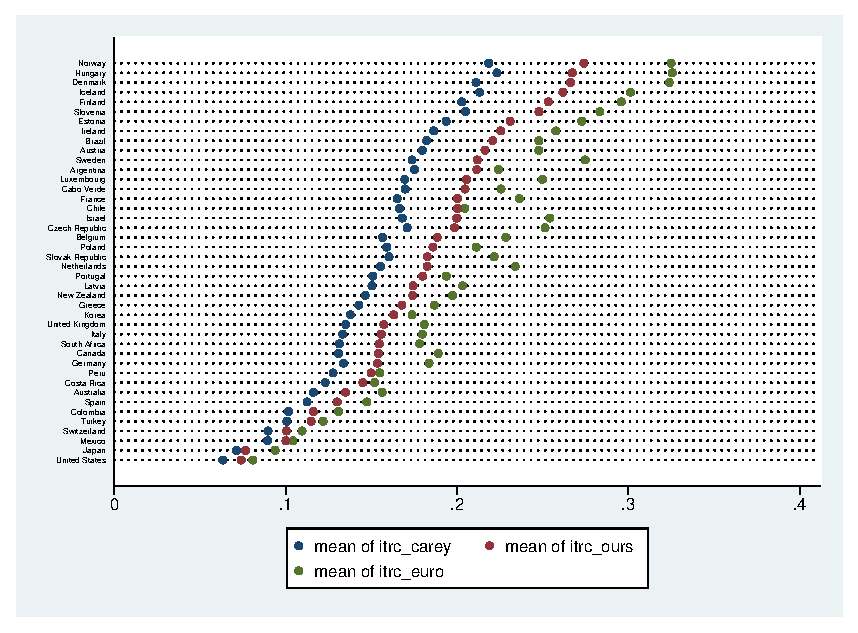
\includegraphics[width=0.9\textwidth]{images/18-09_itrc_comparison}
\caption{Mean of implicit tax rates on consumption for each country.}
\label{fig:itrc_comparison}  
\end{figure}

There are three main definitions for computing implicit effective tax rates on consumption in the economic literature, as described in \cite{euro2016taxation, mendoza1994effective, carey2000average}. We draw on those works in order to propose the following definition:
\[ \tau_{c,y} = \frac{consumption\ taxes\ revenue}{C - CGW - R } \]
where $consumption\ taxes\ revenue$ includes all revenue from consumption taxes, including value-added-taxes (or sales taxes if applicable), excise taxes, taxes on specific services, etc. $C = CP + CG$ is the total final consumption expenditure (private consumption and consumption of general government). $CGW$ is the amount of wages of employees paid by general government, and $R = R_{actual} + R_{imputed} =$ are actual and imputed rentals for housing.

The different possible definitions of implicit tax rates rely on different definitions of the taxable consumption. For example, the definition in \cite{euro2016taxation} relies on a narrower taxable basis, constituted only of private consumption
\begin{equation}
    \label{itrc_euro}
    \tau_{c,y} = \frac{consumption\ taxes\ revenue}{CP}
\end{equation}
while the definition in \cite{carey2000average} considers a broader definition, by taking all consumption
\begin{equation}
    \label{itrc_carey}
    \tau_{c,y} = \frac{consumption\ taxes\ revenue}{C}
\end{equation}

The choice of removing or not rents from the denominator depends on the definition of taxable consumption in micro-data. Since we account for the fact that rents are not subject to consumption taxes by removing rents from the micro-data on consumption, we subtract rents from the denominator of the implicit tax rate. If we do the same for the two alternative definitions described earlier, our definition of implicit tax rates on consumption is thus structurally bounded above by the tax rate under definition \eqref{itrc_euro} and below by that under definition \eqref{itrc_carey} (see \cref{fig:itrc_comparison}). These alternative definitions can be used to produce robustness checks.

\subsection{Estimated regressivity is mitigated when taking rents into account}
\label{sec:rents}
\begin{figure}[!h]
\centering
\includegraphics[height=0.4\textheight]{images/18-11-18_total_nonrent_propensity_fr10}
\caption{Rents represent a higher share of consumption at the bottom of the income distribution (France 2010)}
\label{fig:total_nonrent}  
\end{figure}

Our method allows to account for the fact that housing rentals are not subject to consumption taxes. They are an important part of households' consumption, and they represent a higher share of consumption for poorer households (\cref{fig:total_nonrent}). As a result, the downward slope of propensities to consume are less pronounced when rents are removed from the total amount of consumption. Therefore, we can conclude that micro-simulation methods which apply tax rates on the whole consumption (rent or not) are slightly overestimating the regressivity of consumption taxes.

In order to maximize our coverage of countries and years, we also define another version of the effective tax rate, where actual rentals are not removed from private consumption at the denominator. This definition will be used when micro-data on consumption is not separable between rentals and the rest of the consumption. This smaller rate will be applied on a bigger amount of consumption.
\[ \tau_{wr}= \frac{consumption\ taxes\ revenue}{CP - R_{imputed} + CG - CGW}\]

As shown in \cref{fig:kakrent}, estimated regressivity is reduced when rents are taken into account, and removed from the amount of consumption: the absolute value of the Kakwani index of regressivity can be reduced by up to 20\% for some countries.

\begin{figure}
\centering
\includegraphics[width=0.9\textwidth]{images/18-03-18_kak_kak_wor_mean}
\caption{\label{fig:kakrent} Mean value of Kakwani index whether taxable consumption includes rentals}
\end{figure}

\subsection{Progressive consumption tax rates: test of the bundle effect}
\label{sec:diff_rates}  
Many countries enforce reduced VAT rates for some goods, either in order to boost some economic sectors or to lighten the amount of consumption taxes paid by least affluent households. On the other hand, some goods are more heavily taxed, such as oil or alcohol.

These variations on statutory tax rates can affect the overall progressivity of the tax, as the baskets of goods are different at one point or another of the income distribution. As a robustness check, we design two scenarios, where the effective tax rate is increasing with income. These situations would occur if tax rates had been specifically designed to make consumption taxes more progressive, as it is generally the case. These scenarios introduce a deviation from the median effective tax rate that depends linearly on the percentile of income. In the intermediate scenario, the first percentile of income enjoys an 0.5 percentage points lower effective tax rate than the median household, while the last percentile faces a 0.5 points higher tax rate, so that there is a 1 percentage point difference between the effective tax rate paid by poorest households and richest households. We also provide an extreme scenario where the gap between effective consumption tax rates at both ends is 2 percentage points. Those gaps are in accordance with national case studies that compute effective tax rates depending on income. %TODO : ajouter référence sur les effective tax rates selon décile

We show in \cref{fig:diff_rates} the distribution of tax-to-income ratios by percentiles of income. This allows to compare different situations, from the least progressive to the more progressive. In the first situation, we assume that all goods and services (including housing) would be taxed at the same effective tax rates for all households. The regressive pattern then comes exclusively from the propensity to consume. In the second curve, consumption taxes are applied only on non-housing consumption, which mitigates the regressive pattern (as seen in \cref{sec:rents}). The third and fourth curves introduce progressive consumption taxes according to the intermediate and extreme scenarios.

The curves are very close to one another: this confirms that the ` propensity to consume'' effect is the first order effect. Indeed, simulating an aggregated amount of consumption for each household allows to capture most of the regressivity of consumption taxes. When added the fact that housing consumption is not uniformly distributed, a uniform effective tax rate is even closer to the two scenarios of progressive tax rates.

Eventually, the first and last curves yield upper and lower bounds for the regressivity of consumption taxes. Indeed, we know that using the same effective tax rate for every household, and not taking into account the fact that housing is not subject to consumption taxes actually yields an overestimation of the regressivity of consumption taxes. On the other hand, when we take housing rentals into account and we apply a strong progressivity to effective consumption tax rates, we know that this yields a lower bound of the regressive effect. We can observe that even in the extreme scenario, tax-to-income ratios still present a strong regressive pattern.

The same can be said when looking at measures of redistribution and inequality. \Cref{fig:sum_diff_rates} shows that a constant effective tax rate on whole consumption produces the highest post-tax Gini index (overestimating the eventual income inequality). Adding the information on rent captures most of the difference between the latter and both progressive scenarios. In every case, we observe that all those measures of post-tax income inequality are much closer to one another than to the inequality of disposable income. Qualitatively, the anti-redistributive effect stays significant, and the first and simplest measure provides a quite tight upper bound.

\begin{figure}[!ht]
\centering
\includegraphics[height=0.45\textheight]{"images/20-01 diff_rates"}
\caption{Tax-to-income ratios for France 2010. Medium scenario: 1 pct point difference between effective consumption tax rates of the richest and the least affluent. Extreme scenario: 2 pct points difference}
\label{fig:diff_rates}  
\end{figure}

\begin{figure}[!h]
\centering
\includegraphics[width=0.90\textwidth]{"images/19-11_fr10_sum_diff_rates"}
\caption{Gini indices of income inequality for France 2010. Medium scenario: 1 pct point difference between effective consumption tax rates of the richest and the least affluent. Extreme scenario: 2 pct points difference}
\label{fig:sum_diff_rates}  
\end{figure}

\subsection{Imputation error on consumption depending on the model}
\label{sec:compare_models}
\Cref{fig:compare_models} shows the R2 coefficient for 57 countries-years where imputed and observed values of consumption can be compared. Out of the 57 country-years for which we impute consumption both with \eqref{equ:mod1} and \eqref{equ:mod2}, we observe that model 2 increases the explained variance for 54 of them. On average, it is increased by 33\%, as measured by the R2 coefficient. Overall, the R2 coefficient for model 2 is 0.45 on average, being larger than 0.36 for 75\% of country-years, and larger than 0.56 for a quarter of our observations.

This shows that the independent variable ``cost of housing'', which is the main difference between the two models, provides significant additional information for the imputation of the households' consumption.

\begin{figure}[!h]
\centering
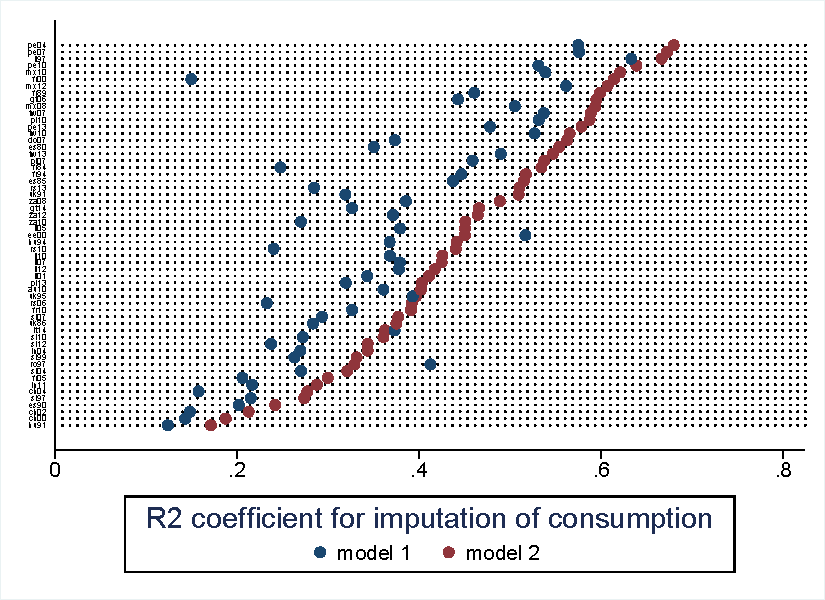
\includegraphics[width=\textwidth]{images/19-04-05_R2_compare_models}
\caption{Explained variance in the two models for various countries}
\label{fig:compare_models}  
\end{figure}

\section{Decomposition of redistributive effect}

\subsection{Vertical and horizontal redistribution}
\label{sec:decomposition}
Effective redistribution can be decomposed into vertical redistribution, measured by the Reynolds-Smolensky index ($RS$), and horizontal redistribution, measured by the reranking index ($Re$):
\begin{equation}
 \label{equ:g_diff}
    \Delta G = G_{dhi} - G_{dhi-tax}  = RS - Re
\end{equation}

Vertical redistribution relates to the amount of tax that is distributed in a progressive or regressive way related to income. A measure of vertical redistribution, the Reynolds-Smolensky index, is defined as follows [reference à ajouter]:
\[ RS = G_{dhi} - C(dhi-tax, dhi) \]
where $G_{dhi}$ is the Gini index of the pre-tax income, while $C(dhi-tax,dhi)$ is the concentration index of the post-tax income ordered on the pre-tax income. This term is thus relatively close to the Gini index of the post-tax income.

Horizontal redistribution is the amount of redistribution that is orthogonal to the distribution of income. The reranking index of horizontal redistribution is a measure of the amount of redistribution that is not due to the regressivity of the tax, but rather an inequality that is created between individuals in the same range of income. It is defined as follows:
\[ Re = G_{dhi-tax} - C(dhi-tax,dhi) \]

By definition, the reranking $Re$ is non-negative, so by \cref{equ:g_diff} the Reynolds-Smolensky index is an upper bound for effective redistribution, and it is a measure of the maximum reachable redistribution if no reranking was entailed by consumption taxes. In our case, if redistribution is negative, then the RS index is a lower bound for the anti-redistributive effect (in absolute value). The rise in income inequality due to taxes is thus the sum of the vertical anti-redistribution (due to the regressive pattern) and the reranking due to the variation in propensities to consume between households of same levels of income. In practice, the Reynolds-Smolensky index is close to the difference in Gini coefficients (see \cref{fig:reranking}): the reranking generally accounts for less than 20\% of the redistributive impact. 

\begin{figure}
    \centering
    \includegraphics[width=\textwidth]{images/19-02_decomposition_effective_redistribution}
    \caption{Decomposition of redistributive effect}
    \label{fig:reranking}
\end{figure}


\subsection{Kakwani indices of regressivity}
\label{sec:kakwani}

We have seen in \cref{equ:decomp_RS} that the vertical redistribution operated by consumption taxes can be viewed as the product of two independent terms: the regressivity, a micro-level term linked to propensities to consume decreasing with income, and the rate of consumption taxes, a macro-level term.

We use the Kakwani index as an index of regressivity of consumption taxes. This indicator is a measure of how concentrated taxes are on one end of the income distribution or the other. It is equal to the difference between the concentration index of the tax relatively to (pre-tax) income and the Gini coefficient of the income [référence à ajouter]. Namely:
\[ Kakwani(tax, dhi) = C(tax,dhi) - Gini(dhi) \]

The concentration index $C(tax,dhi)$ is a measure of how much the distribution of the tax payments is skewed towards highest incomes. The range of its values is [-1;1], -1 indicating that all the tax payments are concentrated on the one poorest individual, while 1 indicates that all the tax payments are concentrated on the richest individual. The computation of this concentration index does not take into account the level of initial income inequality. By substracting the Gini index of income, the Kakwani index provides simple information, based on its sign: if the Kakwani index is positive, it means that the tax payments are more heavily concentrated towards the highest percentiles of income than income itself, meaning that the tax is progressive. On the contrary, if the Kakwani index is negative, then the distribution of tax payments is less skewed to the right than the distribution of income, meaning that the tax is regressive. We are thus expecting negative Kakwani indices.

For one fixed tax rate, we can make assumptions on the Kakwani index and thus have a range of possible RS index values. When the Kakwani indices are derived from imputed consumption values, this will be useful to provide lower and upper bounds on the possible RS values.

We compute the Kakwani index for all the datasets where consumption data is available (i.e.\ 77 country-years), the results are summed up in \cref{fig:kakwani_boxplot}. Approximately half of Kakwani indices lie between -0.10 and -0.15, while almost all of them lie between -0.05 and -0.20.
\begin{figure}
    \centering
    \includegraphics{images/boxplot_kakwani.png}
    \caption{Boxplot of the Kakwani indices}
    \label{fig:kakwani_boxplot}
\end{figure}

Based on the different tax rates that we have computed earlier, we are now able to frame the possible values of the RS index. As summed up in \cref{fig:RS_scenarii}, most values for the Reynolds-Smolensky index will lie between -0.02 and -0.08.
\begin{figure}
	\centering
	\includegraphics[scale=0.8]{images/18-12_RS_scenarii}
	\caption{Value of Reynolds-Smolensky index depending on tax rate and Kakwani index}
	\label{fig:RS_scenarii}
\end{figure}

\section{Country and years coverage}
\label{A-datasets}
We select a total of \textbf{216} LIS datasets. 

In \cref{tab:datasets}, countries marked with an \textbf{(R)} are used in the regression pool. For years marked with an *, information on rents is missing.

\begin{tabularx}{\textwidth}{lXX}
        \caption{Country and years used in the study} \\
\hline
Country            & Years with observed data                       & Years with imputed data                                       \\ \hline
Australia \textbf{(R)}      & 2010*                                          & 1989, 1995, 2001, 2003, 2008                                  \\
Austria            &                                                & 1994, 1995, 1997, 2000, 2004, 2007, 2010, 2013                \\
Belgium            &                                                & 1992, 1995, 1997*, 2000                                       \\
Brazil             &                                                & 2006, 2009, 2011, 2013                                        \\
Colombia           &                                                & 2007, 2010, 2013                                              \\
Czech Republic     &                                                & 2004, 2007, 2010, 2013                                        \\
Denmark            &                                                & 1987*, 1992, 2000, 2004, 2007*, 2010*, 2013*                  \\
Dominican Republic & 2007                                           &                                                               \\
Estonia            & 2000                                           & 2004, 2007, 2010, 2013                                        \\
Finland            &                                                & 1987*, 1991, 1995*, 2000*, 2004*, 2007*, 2010*, 2013*         \\
France \textbf{(R)}         & 1984, 1989, 1994, 2000, 2005, 2010             &                                                               \\
Germany            &                                                & 1984, 1989, 1994, 2000, 2004, 2007, 2010, 2013                \\
Greece             &                                                & 2004, 2007, 2010, 2013                                        \\
Guatemala          & 2006, 2014                                     & 2011                                                          \\
Hungary \textbf{(R)}        & 1991, 1994, 1999, 2005, 2007, 2009, 2012       &                                                               \\
Iceland            &                                                & 2004, 2007, 2010                                              \\
India              & 2004, 2011                                     &                                                               \\
Ireland            &                                                & 1994, 1995, 1996, 2000, 2004, 2007, 2010                      \\
Israel             & 2001, 2005, 2007, 2010, 2012                   & 1979*                                                         \\
Italy \textbf{(R)}          & 1995*, 1998*, 2000*, 2004*, 2008*, 2010*, 2014 & 1986*, 1987, 1989, 1991, 1993                                 \\
Japan              &                                                & 2008                                                          \\
Luxembourg         &                                                & 1991, 1994, 1997, 2000, 2007, 2010, 2013                      \\
Mexico             & 2008, 2010, 2012                               & 1984*, 1989*, 1992*, 1994*, 1996*, 1998*, 2000*, 2002*, 2004* \\
Netherlands        &                                                & 1983*, 1987, 2004, 2007, 2010, 2013                           \\
Norway             &                                                & 1979*                                                         \\
Panama             &                                                & 2010, 2013                                                    \\
Paraguay           &                                                & 2010, 2013                                                    \\
Peru               & 2004, 2007, 2010, 2013                         &                                                               \\
Poland \textbf{(R)}         & 2007, 2010, 2013                               & 1986*, 1995*, 1999*, 2004*                                    \\
Russia             & 2000, 2004, 2007, 2010, 2013                   &                                                               \\
Serbia             & 2006, 2010, 2013                               &                                                               \\
Slovakia           &                                                & 2004, 2007, 2010, 2013                                        \\
Slovenia \textbf{(R)}       & 1997, 1999, 2004, 2007, 2010, 2012             &                                                               \\
Spain \textbf{(R)}          & 1980, 1990                                     & 1995, 2000, 2004, 2007, 2010, 2013                            \\
Sweden             &                                                & 2000, 2005                                                    \\
Switzerland        &                                                & 1982*, 1992, 2007, 2010, 2013                                 \\
Taiwan \textbf{(R)}         & 1981, 1986, 1991, 2007, 2010, 2013             & 1995*, 1997*, 2000*, 2005*                                    \\
United Kingdom \textbf{(R)} & 1986, 1991, 1995                               & 1994, 1999, 2004, 2007, 2010, 2013                            \\
United States      &                                                & 1979, 1986, 1991, 1994, 1997, 2000, 2004, 2007, 2010, 2013    \\
Uruguay            &                                                & 2004*, 2007, 2010, 2013                                       \\ \hline
    \label{tab:datasets}
    
\end{tabularx}



\end{document}
